\chapter{Identification and validation}
 \label{sec:identification and validation}

 The model verification addresses the question whether the implemented model as a whole and its components conceptionally meet its criteria. 
 %
 According to the aim of the simulation that is to model the reality as perfect as possible, a real scenario in the simulation environment is exactly reproduced, including the elimination of errors in the model and the fine tuning of the parameters that were not available in the literature or through measurements. 
 %
 Considering the manufacturing and measurement tolerances, the model and the simulation will never be exactly the same. The claim for the simulation should thus be the qualitatively correct depiction of the trend shown by the real measurement. 
 
 Here the validation consist of two parts: Firstly, the identification of the damping coefficient and validation of the time response while traversing the speed bump with different velocities. Secondly, the identification of the parameters for formula~\ref{form:K} and validation of the vehicle vibration while traversing different obstacles with different velocities.
 %
 The real measurements are performed with a BMW 116d.
 
 
 \section{Identification and validation of the damping ratio}
 
 In one of the real measurements the vehicle drives at the speed of $20km/h$ across a speed bump which is $13mm$ high and $70mm$ wide on only one side of the road and the sensor is in the glove compartment (S4 in Sec.~\ref{sec:positionofoutput}). 
 %
 According to the principle of the validation, the situation should be identically reproduced in the simulation. 
 %
 The \ac{FCM} which will be used in the validation is with the basic point contact tire model because the parameter in \ref{form:K} is till unknown.
 %
 As what is mentioned in Sec.~\ref{sec:tire_model}, the point contact tire model performs good only when the wavelength of the obstacle greater than the contact patch, which is about $150mm$ long.
 
 Fig.~\ref{fig:tire_bump} shows the geometric relationship when the tire just meets the speed bump.
 %
 It can be seen that the tire has already touched the speed bump before the vehicle arrives the start point of it ($C$).
 %
 Hence in the simulation the start point of the speed bump should be at $D$, not $C$.
 %
 On the basis of the trigonometric function it is known that

 \begin{align}
    |AC|&=\sqrt{|AB|^2+|BC|^2}=\sqrt{13^2+(70/2)^2}mm = 37.4mm \\
    \angle A &= arctan(\frac{|BC|}{|AB|}) = \ang{70} \\
    \angle O_2&= \pi - 2*\angle A = \ang{40}
 \end{align}
 
 With the law of sines,
 \begin{equation}
    \frac{|AC|}{\angle O_2} = \frac{r_2}{\angle A}
 \end{equation} 
 
 Thus $r_2 = 53.6mm$.
 
 The radius of tire $r_1$ can be read from the sidewall of the tire. 
 %
 From the last dimension listed in the size number '195/55R16' it is known that the diameter of the wheel rim is 16 inch.
 %
 According to \cite{Tire_calculator} the diameter of the tire $r_1$ is about $660mm$.
 
 It is easy to calculate the length $|O_2D| \doteq 100mm$.
 %
 Hence the complete length of the speed bump in the simulation should be $2\cdot |O_2D| = 200mm$, which is greater than the contact patch.
 %
 It means the use of the basic point contact tire model is feasible in this situation.
 
 The speed bump is modeled by a sine function which is shown in Fig.~\ref{fig:bump}.
 %
 Addition to the roughness of the asphalt surface ($IRI=1$), the road model is created.
 %
 Tuning the damping ratio of the suspensions to get the results that is most similar to the actual measurement, including the peak of the amplitude and the duration of the vibration.
 
 \begin{figure}
 \centering
 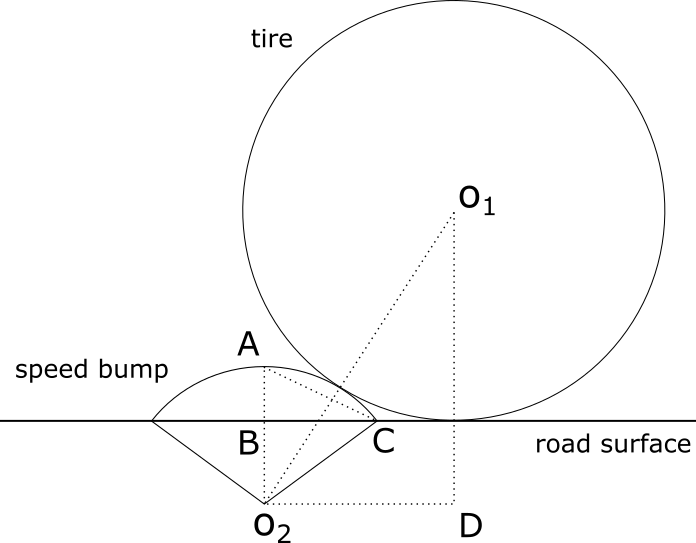
\includegraphics[width=0.5\textwidth]{bilder/validation.png}
 \caption{Geometric of the tire and speed bump.}
 \label{fig:tire_bump}
 \end{figure}
 
 
 
 \begin{figure}
 \centering
 \begin{tikzpicture}
 \begin{groupplot}[mygroupplot,
 group style={group name=my plots,group size= 1 by 1, horizontal sep=\myGroupSep,vertical sep=\myGroupVertSep},
 ]
 		
 	\nextgroupplot[
	ylabel= Height ($m$),
	xlabel= Length ($m$),
	%xmin=27,   
	%xmax=93,
   	ymin=0,   
   	%ymax=1.4,
% 	legend columns=1,
% 	legend entries={center of gravity, middle of left side},
% 	legend style={at={\myLegendPosition},anchor=south,name=leg},
    cycle list name=mycyclelist,
    ]
    \newcommand{\point}{1};
    \addplot+[no marks, each nth point=\point] table[x=r,y=h] {data/speed_bump.txt};
 
 \end{groupplot}
 \end{tikzpicture}
 \label{fig:bump}
 \caption{Profile of the simulated speed bump.}
 \end{figure}

 
 
 \begin{figure}
 \centering
 \begin{tikzpicture}
 \begin{groupplot}[mygroupplot,
 group style={group name=my plots,group size= 2 by 3, horizontal sep=\myGroupSep},
 ]
 		
 	\nextgroupplot[
	ylabel=Vertical acceleration ($g$),
	%xmin=27,   
	%xmax=93,
   	ymin=0.6,   
   	ymax=1.4,
% 	legend columns=1,
% 	legend entries={center of gravity, middle of left side},
% 	legend style={at={\myLegendPosition},anchor=south,name=leg},
    cycle list name=mycyclelist,
    ]
    \newcommand{\point}{1};
    \addplot+[no marks, each nth point=\point] table[x=x1,y=y3] {data/P3_20_Links3.txt};
    
    \nextgroupplot[
	%xmin=27,   
	%xmax=93,
   	ymin=0.6,   
   	ymax=1.4,
% 	legend columns=1,
% 	legend entries={center of gravity, middle of left side},
% 	legend style={at={\myLegendPosition},anchor=south,name=leg},
    cycle list name=mycyclelist,
    ]
    \newcommand{\point}{1};
    \addplot+[no marks, each nth point=\point] table[x=t,y=z] {data/validation_measure_data.txt};
    
    \nextgroupplot[
	%xlabel=Time ($s$),
	ylabel=Roll rate ($rad/s$),
	%xmin=27,   
	%xmax=93,
   	ymin=-0.04,   
  	ymax=0.06,
% 	legend columns=1,
% 	legend entries={center of gravity, middle of left side},
% 	legend style={at={\myLegendPosition},anchor=south,name=leg},
    cycle list name=mycyclelist,
    ]
    \newcommand{\point}{1};
    \addplot+[no marks, each nth point=\point] table[x=x1,y=y4] {data/P3_20_Links3.txt};
    
    \nextgroupplot[
	%xlabel=Time ($s$),
	%xmin=27,   
	%xmax=93,
    ymin=-0.04,   
  	ymax=0.06,
% 	legend columns=1,
% 	legend entries={center of gravity, middle of left side},
% 	legend style={at={\myLegendPosition},anchor=south,name=leg},
    cycle list name=mycyclelist,
    ]
    \newcommand{\point}{1};
    \addplot+[no marks, each nth point=\point] table[x=t,y=r] {data/validation_measure_data.txt};
    
    \nextgroupplot[
	xlabel=Time ($s$),
	ylabel=Pitch rate ($rad/s$),
	%xmin=27,   
	%xmax=93,
   	ymin=-0.04,   
  	ymax=0.04,
% 	legend columns=1,
% 	legend entries={center of gravity, middle of left side},
% 	legend style={at={\myLegendPosition},anchor=south,name=leg},
    cycle list name=mycyclelist,
    ]
    \newcommand{\point}{1};
    \addplot+[no marks, each nth point=\point] table[x=x1,y=y5] {data/P3_20_Links3.txt};
    
    \nextgroupplot[
	xlabel=Time ($s$),
	%xmin=27,   
	%xmax=93,
    ymin=-0.04,   
  	ymax=0.04,
% 	legend columns=1,
% 	legend entries={center of gravity, middle of left side},
% 	legend style={at={\myLegendPosition},anchor=south,name=leg},
    cycle list name=mycyclelist,
    ]
    \newcommand{\point}{1};
    \addplot+[no marks, each nth point=\point] table[x=t,y=p] {data/validation_measure_p.txt};
 
 \end{groupplot}
 
 \node[below = \myLabelSep of my plots c1r3.south] {(a) real measurements};
 \node[below = \myLabelSep of my plots c2r3.south] {(b) simulation};
 
 \end{tikzpicture}
 \label{fig:validation_bump}
 \caption{Comparison of the vehicle response to a speed bump.}
 \end{figure}
 

The identified coefficient of the damping is shown in table~\ref{tbl:damping}.
%
With those coefficient the comparison between the measured data and the simulation is shown in Fig.~\ref{fig:validation_bump}.
% 
It can be seen that although the value of the peaks do not complete match the reality, the general behaviour of the simulation is very similar to the actual measurement, which validates that the \ac{FCM} can correctly simulate the behaviour of a real vehicle.

\begin{table}
\centering
\caption{Stiffness and damping ratio of the full car model.}
\label{tbl:damping}
\begin{tabular}{lcccccccc}
\hline
variable & $k_1$ & $k_2$ & $k_3$ & $k_4$ & $d_1$ & $d_2$ & $d_3$ & $d_4$ \\
unit & \multicolumn{4}{c}{$[kN\cdot m^{-1}]$} & \multicolumn{4}{c}{[$kN\cdot s \cdot m^{-1}]$} \\
value & 16 & 16 & 16 & 16 & 1 & 1 & 1 & 1 \\ \hline
\end{tabular}
\end{table}
 
 
 
 
 
 
 \section{Identification and validation of the tire model}
 
 
 \begin{table}
 \centering
 \caption{Parameters for $K$ and size of different events.}
 \label{tbl:parameter of K}
 \begin{tabular}{lllllll}
 \hline
 events & $a_0$ & $a_1$ & $a_2$ & $a_3$ & $l/[m]$ & $h/[m]$ \\ \hline
 pothole & 0 & 0.03 & 1 & 1 & 0.5 & 0.02\\
 manhole cover & 0 & 0.015 & 0 & 1 & 0.5 & 0.01 \\
 cobbled road & 0 & 0.04 & 1 & 1 & 0.2 & 0.02 \\
 railway crossing & 0.02 & 0 & 0 & 0 & 1.45 & 0.1\\ \hline
 \end{tabular}
 \end{table}
 
 
 \begin{figure}
 \centering
 \begin{tikzpicture}
 \begin{groupplot}[mygroupplot,
 group style={group name=my plots,group size= 2 by 3, horizontal sep=\myGroupSep,vertical sep=\myGroupVertSep}]
 		
 	\nextgroupplot[
	ylabel=$\sigma$(vertical acceleration) ($m/s^2$),
	%xmin=27,   
	%xmax=93,
   	ymin=0,   
   	ymax=0.4,
   	cycle list name=mycyclelist,
    ]
    \newcommand{\point}{1};
    \addplot+[error bars/.cd, y dir=both,y explicit]
    coordinates {
    (8.3,0.027) +- (0.00085,0.00085)
    (11.1,0.036) +- (0.009,0.009)
    (13.9,0.0396) +- (0.0007,0.0007)
    (16.7,0.0476) +- (0.0012,0.0012)};
    %\addlegendentry{Asphalt}
    
    \addplot+[error bars/.cd, y dir=both,y explicit]
    coordinates {
    (8.3,0.04) +- (0.0005,0.0005)
    (11.1,0.046) +- (0.0037,0.00037)
    (13.9,0.048) +- (0.0035,0.0035)
    (16.7,0.05) +- (0.0041,0.0041)};
    %\addlegendentry{Railroad crossing}
    
    \addplot+[error bars/.cd, y dir=both,y explicit]
    coordinates {
    (8.3,0.045) +- (0.0034,0.0034)
    (11.1,0.059) +- (0.0036,0.0036)
    (13.9,0.074) +- (0.003,0.003)
    (16.7,0.1) +- (0.0028,0.0028)};
   % \addlegendentry{Manhole cover}

    \addplot+[error bars/.cd, y dir=both,y explicit]
    coordinates {
    (8.3,0.129) +- (0.0039,0.0039)
    (11.1,0.161) +- (0.0029,0.0029)
    (13.9,0.168) +- (0.001,0.001)
    (16.7,0.177) +- (0.0015,0.0015)};
    %\addlegendentry{Cobbled road}

    \addplot+[error bars/.cd, y dir=both,y explicit]
    coordinates {
    (8.3,0.18) +- (0.0072,0.0072)
    (11.1,0.28) +- (0.014,0.014)
    (13.9,0.3) +- (0.025,0.025)
    (16.7,0.3) +- (0.012,0.012)};
   % \addlegendentry{Pothole}

    \addplot+[error bars/.cd, y dir=both,y explicit]
    coordinates {
    (8.3,0.116) +- (0.0041,0.0041)
    (11.1,0.142) +- (0.0017,0.0017)
    (13.9,0.164) +- (0.0023,0.0023)
    (16.7,0.184) +- (0.002,0.002)};
    %\addlegendentry{Unevennesses}
    
    \nextgroupplot[
	%ylabel=$\sigma$(vertical acceleration) ($m/s^2$),
	%xmin=27,   
	%xmax=93,
   	ymin=0,   
   	ymax=0.4,
   	legend columns=3,
  	legend style={at={(-0.3,1.03)},anchor=south,name=leg},
  	cycle list name=mycyclelist,
    ]
    \newcommand{\point}{1};
    \addplot+[error bars/.cd, y dir=both,y explicit]
    table[x = v, y = m1, y error = e1]{data/ddz_obstacles_velocity.txt};
    \addlegendentry{asphalt}
    
    \addplot+[error bars/.cd, y dir=both,y explicit]
    table[x = v, y = m2, y error = e2]{data/ddz_obstacles_velocity.txt};
    \addlegendentry{railroad crossing}
    
    \addplot+[error bars/.cd, y dir=both,y explicit]
    table[x = v, y = m3, y error = e3]{data/ddz_obstacles_velocity.txt};
    \addlegendentry{manhole cover}

    \addplot+[error bars/.cd, y dir=both,y explicit]
    table[x = v, y = m4, y error = e4]{data/ddz_obstacles_velocity.txt};
   \addlegendentry{cobbled road}

    \addplot+[error bars/.cd, y dir=both,y explicit]
    table[x = v, y = m5, y error = e5]{data/ddz_obstacles_velocity.txt};
   \addlegendentry{pothole}

    \addplot+[error bars/.cd, y dir=both,y explicit]
    table[x = v, y = m6, y error = e6]{data/ddz_obstacles_velocity.txt};
   \addlegendentry{unevenness}
    
    \nextgroupplot[
	%xlabel=Velocity ($m/s$),
	ylabel=$\sigma$(roll rate) ($rad/s$),
	%xmin=27,   
	%xmax=93,
   	ymin=0,   
   	ymax=0.05,
% 	legend columns=1,
% 	legend entries={center of gravity, middle of left side},
% 	legend style={at={\myLegendPosition},anchor=south,name=leg},
    cycle list name=mycyclelist,
    ]
    \newcommand{\point}{1};
    \addplot+[error bars/.cd, y dir=both,y explicit]
    coordinates {
	(8.3,0.0034) +- (0.00014,0.00014)
	(11.1,0.0040) +- (0.000082,0.000082)
	(13.9,0.00453) +- (0.000062,0.000062)
	(16.7,0.0061) +- (0.00027,0.00027)};
	%\addlegendentry{Asphalt}
 
    \addplot+[error bars/.cd, y dir=both,y explicit]
    coordinates {
    (8.3,0.0081) +- (0.0006,0.0006)
    (11.1,0.0088) +- (0.00027,0.00027)
    (13.9,0.008) +- (0.00055,0.00055)
    (16.7,0.0088) +- (0.00044,0.00044)};
    %\addlegendentry{Railroad crossing}
    
    \addplot+[error bars/.cd, y dir=both,y explicit]
    coordinates {
    (8.3,0.00945) +- (0.00027,0.00027)
    (11.1,0.0139) +- (0.00064,0.00064)
    (13.9,0.015) +- (0.0011,0.0011)
	(16.7,0.028) +- (0.00028,0.00028)};
	%\addlegendentry{Manhole cover}
	
	\addplot+[error bars/.cd, y dir=both,y explicit]
	coordinates {
	(8.3,0.0192) +- (0.0003,0.0003)
	(11.1,0.024) +- (0.00045,0.00045)
	(13.9,0.0275) +- (0.00022,0.00022)
	(16.7,0.0299) +- (0.00033,0.00033)};
	%\addlegendentry{Cobbled road}
	
	\addplot+[error bars/.cd, y dir=both,y explicit]
	coordinates {
	(8.3,0.0288) +- (0.00045,0.00045)
	(11.1,0.036) +- (0.0011,0.0011)
	(13.9,0.046) +- (0.0008,0.0008)
	(16.7,0.04) +- (0.0002,0.0002)};
	%\addlegendentry{Pothole}
	
	\addplot+[error bars/.cd, y dir=both,y explicit]
	coordinates {
	(8.3,0.0187) +- (0.00012,0.00012)
	(11.1,0.0224) +- (0.0004,0.0004)
	(13.9,0.0245) +- (0.00027,0.00027)
	(16.7,0.027) +- (0.0005,0.0005)};
	%\addlegendentry{Unevennesses}
	
	\nextgroupplot[
	%xlabel=Velocity ($m/s$),
	%ylabel=$\sigma$(roll rate) ($rad/s$),
	%xmin=27,   
	%xmax=93,
   	ymin=0,   
   	ymax=0.05,
% 	legend columns=1,
% 	legend entries={center of gravity, middle of left side},
% 	legend style={at={\myLegendPosition},anchor=south,name=leg},
    cycle list name=mycyclelist,
    ]
    \newcommand{\point}{1};
    \addplot+[error bars/.cd, y dir=both,y explicit]
    table[x = v, y = m1, y error = e1]{data/ddr_obstacles_velocity.txt};
    %\addlegendentry{Asphalt}
    
    \addplot+[error bars/.cd, y dir=both,y explicit]
    table[x = v, y = m2, y error = e2]{data/ddr_obstacles_velocity.txt};
    %\addlegendentry{Railroad crossing}
    
    \addplot+[error bars/.cd, y dir=both,y explicit]
    table[x = v, y = m3, y error = e3]{data/ddr_obstacles_velocity.txt};
    %\addlegendentry{Manhole cover}

    \addplot+[error bars/.cd, y dir=both,y explicit]
    table[x = v, y = m4, y error = e4]{data/ddr_obstacles_velocity.txt};
    %\addlegendentry{Cobbled road}

    \addplot+[error bars/.cd, y dir=both,y explicit]
    table[x = v, y = m5, y error = e5]{data/ddr_obstacles_velocity.txt};
    %\addlegendentry{Pothole}

    \addplot+[error bars/.cd, y dir=both,y explicit]
    table[x = v, y = m6, y error = e6]{data/ddr_obstacles_velocity.txt};
    %\addlegendentry{Unevennesses}
    
    
     \nextgroupplot[
	xlabel=Velocity ($m/s$),
	ylabel=$\sigma$(pitch rate) ($rad/s$),
	%xmin=27,   
	%xmax=93,
   	ymin=0,   
   	ymax=0.07,
% 	legend columns=1,
% 	legend entries={center of gravity, middle of left side},
% 	legend style={at={\myLegendPosition},anchor=south,name=leg},
    cycle list name=mycyclelist,
    ]
    \newcommand{\point}{1};
    \addplot+[error bars/.cd, y dir=both,y explicit]
    coordinates {
	(8.3,0.0064) +- (0.00003,0.00003)
	(11.1,0.00675) +- (0.0001,0.0001)
	(13.9,0.008) +- (0.0002,0.0002)
	(16.7,0.0097) +- (0.0001,0.0001)};
	%\addlegendentry{Asphalt}
 
    \addplot+[error bars/.cd, y dir=both,y explicit]
    coordinates {
    (8.3,0.011) +- (0.00035,0.00035)
	(11.1,0.0129) +- (0.00039,0.00039)
	(13.9,0.0125) +- (0.00052,0.00052)
	(16.7,0.0113) +- (0.0013,0.0013)};
    %\addlegendentry{Railroad crossing}
    
    \addplot+[error bars/.cd, y dir=both,y explicit]
    coordinates {
    (8.3,0.0167) +- (0.00096,0.00096)
	(11.1,0.0176) +- (0.00021,0.00021)
	(13.9,0.022) +- (0.001,0.001)
	(16.7,0.034) +- (0.001,0.001)};
	%\addlegendentry{Manhole cover}
	
	\addplot+[error bars/.cd, y dir=both,y explicit]
	coordinates {
	(8.3,0.0326) +- (0.0002,0.0002)
	(11.1,0.0355) +- (0.00023,0.00023)
	(13.9,0.0371) +- (0.0003,0.0003)
	(16.7,0.0382) +- (0.00012,0.00012)};
	%\addlegendentry{Cobbled road}
	
	\addplot+[error bars/.cd, y dir=both,y explicit]
	coordinates {
	(8.3,0.051) +- (0.0016,0.0016)
	(11.1,0.061) +- (0.0018,0.0018)
	(13.9,0.065) +- (0.004,0.004)
	(16.7,0.063) +- (0.001,0.001)};
	%\addlegendentry{Pothole}
	
	\addplot+[error bars/.cd, y dir=both,y explicit]
	coordinates {
	(8.3,0.0291) +- (0.00023,0.00023)
	(11.1,0.033) +- (0.0003,0.0003)
	(13.9,0.0373) +- (0.0005,0.0005)
	(16.7,0.041) +- (0.00028,0.00028)};
	%\addlegendentry{Unevennesses}
	
	\nextgroupplot[
	xlabel=Velocity ($m/s$),
	%ylabel=$\sigma$(roll rate) ($rad/s$),
	%xmin=27,   
	%xmax=93,
   	ymin=0,   
   	ymax=0.07,
% 	legend columns=1,
% 	legend entries={center of gravity, middle of left side},
% 	legend style={at={\myLegendPosition},anchor=south,name=leg},
    cycle list name=mycyclelist,
    ]
    \newcommand{\point}{1};
    \addplot+[error bars/.cd, y dir=both,y explicit]
    table[x = v, y = m1, y error = e1]{data/ddp_obstacles_velocity.txt};
    %\addlegendentry{Asphalt}
    
    \addplot+[error bars/.cd, y dir=both,y explicit]
    table[x = v, y = m2, y error = e2]{data/ddp_obstacles_velocity.txt};
    %\addlegendentry{Railroad crossing}
    
    \addplot+[error bars/.cd, y dir=both,y explicit]
    table[x = v, y = m3, y error = e3]{data/ddp_obstacles_velocity.txt};
    %\addlegendentry{Manhole cover}

    \addplot+[error bars/.cd, y dir=both,y explicit]
    table[x = v, y = m4, y error = e4]{data/ddp_obstacles_velocity.txt};
    %\addlegendentry{Cobbled road}

    \addplot+[error bars/.cd, y dir=both,y explicit]
    table[x = v, y = m5, y error = e5]{data/ddp_obstacles_velocity.txt};
    %\addlegendentry{Pothole}

    \addplot+[error bars/.cd, y dir=both,y explicit]
    table[x = v, y = m6, y error = e6]{data/ddp_obstacles_velocity.txt};
    %\addlegendentry{Unevennesses}
 
 \end{groupplot}
 
\node[below = \myLabelSep of my plots c1r3.south] {(a) real measurements};
\node[below = \myLabelSep of my plots c2r3.south] {(b) simulation};
 
 \end{tikzpicture}
 \label{fig:validation_events}
 \caption{Comparison of the standard deviation $\sigma$ of vertical acceleration, roll rate and pitch rate between real measurement and simulated results.}
 \end{figure}
 
 
 
 To identify the parameter in the formula~\ref{form:K}, different obstacles with different wavelength should be tested.
 %
 In the real driving test the the BMW 116d crosses six different events including asphalt road, pothole, manhole cover, railway crossing, cobbled road and evenness at four different velocities form $20km/h$ to $60km/h$
 
 All of the following outputs are measured at the center of gravity. 
 %
 For each velocity and each measuring event four runs are conducted and then the averaged value of the parameter is reported.
 %
 The error bars show the standard deviation of the obtained values.
 
 The best situation is that the modified point contact model can be applied in all different obstacles after the identification.
 %
 However, it hard to fulfill due to the simply structure an principle of the model.
 %
 The dynamic process between the obstacle and tire is so complicated that it is difficult to build a accuracy model with the point contact model an only two variables $e$ and $v$.
 
 Thus, for different obstacles different parameters of formula~\ref{form:K} should be identified separately to describe the real motion of the tire and the road.
 %
 Although the amount of the labor has increased, the results proves to be satisfied. 
 %
 The result of the measured data and the simulation after the identification are shown in Fig.~\ref{fig:validation_events}.
 %
 And the identified parameters of the filer are shown in table~\ref{tbl:parameter of K}. 
 
 It is observed that the simulated results have a very similar distribution as the measured data. 
 %
 Despite some simulated value has a deviation from the real data, the tendency and the relative position of different outputs by different obstacles are in general the same as the results of the measurement.
 %
 These clearly and correctly divided data has a positive influence on the accuracy of the classification.
 
 After the vehicle model and road model have been appropriately identified, the outputs provides not only a generally accuracy of the value e.g. the vertical acceleration, roll rate and pitch rate, also performs a similar features and relations compared with the actual data e.g. the duration of the signal and the standard deviations of different signals.
 
 In conclusion, the data which has been simulated by the road- and vehicle model is proved to be in the line with the facts.
 %
 Thus, the results and accuracy of the data processing in the next chapters shall be reasonable and well-founded.
 
 
 